\section{Исследовательская часть}

В рамках разработки данной АИС были решены следующие задачи:
\begin{itemize}
\item Проектирование алгоритма символьной регрессии на основе эволюционного подхода;
\item Исследование сходимости алгоритма эволюционной регрессии;
\item Исследование закона распределения сходимости алгоритма эволюционной регрессии;
\end{itemize}

\subsection{Описание эволюционного алгоритма символьной регрессии}

Так как результат модуля прогнозирования должен содержать аналитическую формулу прогноза и работать с любыми видами аналитических функций, то для метода прогнозирования хорошо подходит метод символьной регрессии~\cite{SymbolicRegression}.

Общая идея эволюционных алгоритмов~\cite{KozaTheBase} состоит в моделировании процесса естественного отбора, наблюдаемого в природе. Потенциальные решения проблемы представляются в качестве индивидов, подверженных естественному отбору. Каждый индивид имеет набор хромосом, в которых кодируется необходимая информация о данном решении проблемы. Индивиды объединяются в замкнутые популяции, эволюция в разных популяциях идет параллельно, что позволяет находить альтернативные конкурирующие решения задачи.

Для решения задач эволюционными алгоритмами необходимо знать функцию оценки, иначе называемой функцией приспособленности. Данная функция ставит в соответствие каждому индивиду число, отражающего качество решения задачи, записанное в хромосомах индивида:
\begin{equation}
\label{equation:fitness}
fitness : Ind \rightarrow \mathbb{R}
\end{equation}
\begin{ESKDExplanation}
\item[где ] $Ind$ -- множество всех индивидов;
\end{ESKDExplanation}

Эволюционный отбор базируется на применении эволюционных операторов:
\begin{itemize}
\item Мутация -- преобразование хромосом единичного индивида случайным образом. Данный оператор позволяет производить хаотический поиск решений во всем пространстве поиска.
\item Скрещивание -- преобразование хромосом пары индивидов, которые выбираются из популяции в соответствии значениям их функции оценки. Данный оператор работает из предположения, что комбинация хромосом успешных родителей может дать более успешного потомка. Скрещивание помогает находить новые решения путем комбинации уже найденных, но не привносит концептуально новые решения в популяцию.
\item Элитизм -- перенос части лучших индивидов в следующее поколение популяции. Данный оператор позволяет гарантировать неубывающую последовательность лучших решений проблемы из поколения в поколение.
\end{itemize}

Генетический алгоритм в общем виде представлене на рис~\ref{figure:genetics}.

\begin{figure}[h!]
\centering
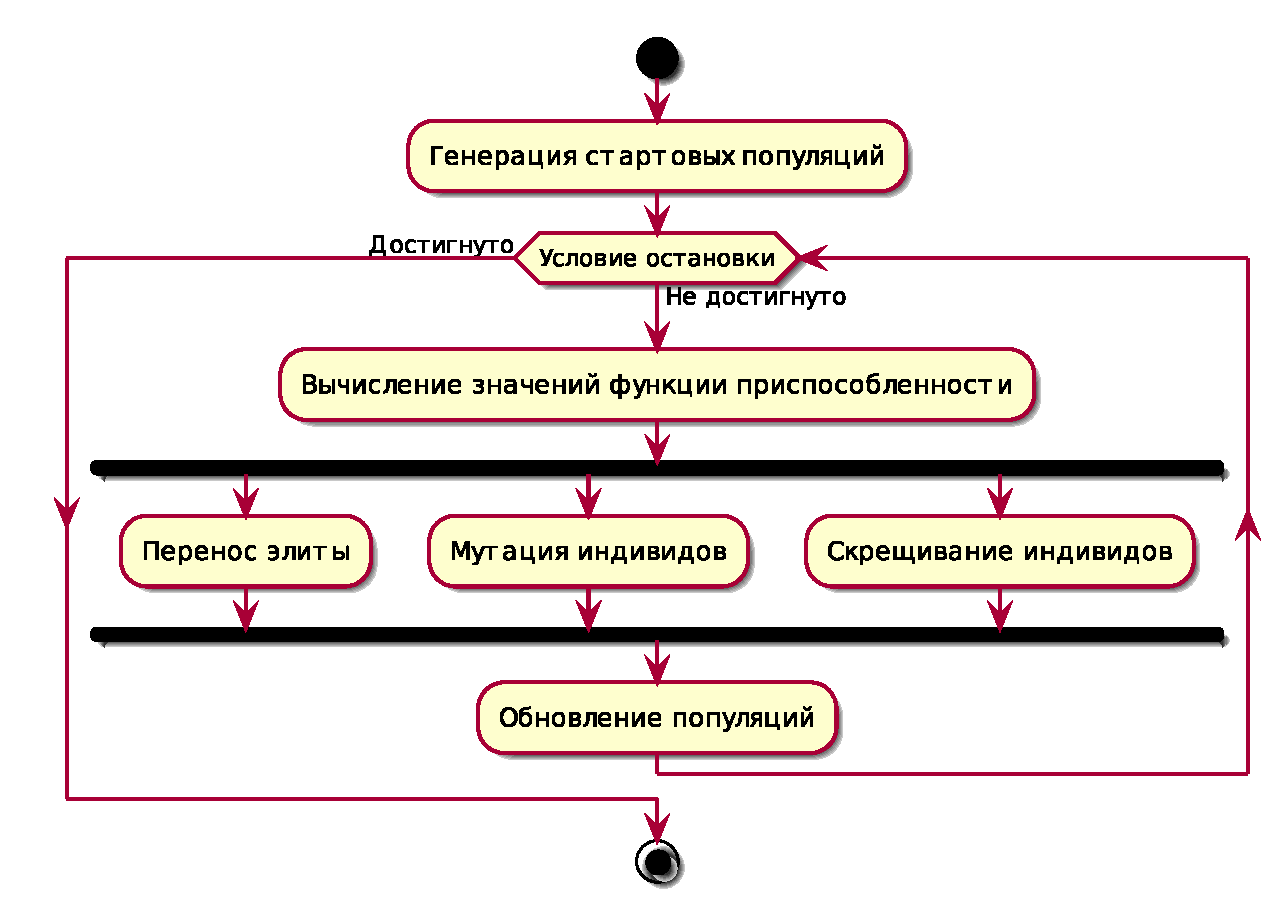
\includegraphics[width=0.5\textwidth]{science/genetic}
\caption{Общая схема генетического алгоритма}
\label{figure:genetics}
\end{figure}

\subsection{Исследование сходимости алгоритма от размера популяции}

Одним из самых важных параметров эволюционного алгоритма является количество индивидов в популяции. Установка данного значения сильно влияет на скорость нахождения решения задачи символьной регрессии. С первого взгляда нельзя сказать, какой размер популяции стоит выбирать, так как малый размер популяции замедляет сходимость из-за малого разнообразия решений в популяции, а чрезмерный размер является избыточным. 

Согласно работе~\cite{PopulationSize} метрикой сходимости генетических алгоритмов может являться количество поколений, необходимое для достижения нужного значения функции приспособленности.

Для экспериментов выберем функцию, которая должна удовлетворять следующим требованиям:
\begin{itemize}
\item Должна представлять типичный временной ряд для новостного потока. По результатам наблюдения за собранными данными, такая функция является периодической, немонотонной, ее значения колеблется в небольших пределах выше 0.
\item Должна быть достаточно сложной, чтобы эволюционный алгоритм с малой вероятностью генерировал правильный ответ при инициализации популяции.
\item Должна быть достаточно простой, чтобы эволюционный алгоритм с ограничением на максимальную глубину синтаксического дерева мог найти подходящую под данные функцию.
\end{itemize}

Выберем функцию:
\begin{equation}
\label{equation:testFunction}
F(x) = sin (2 \cdot x ^ 2) + 2 \cdot cos (10 \cdot x)
\end{equation}

На рис.~\ref{figure:testFunction} представлен график тестовой функции.

\begin{figure}[h!]
\centering
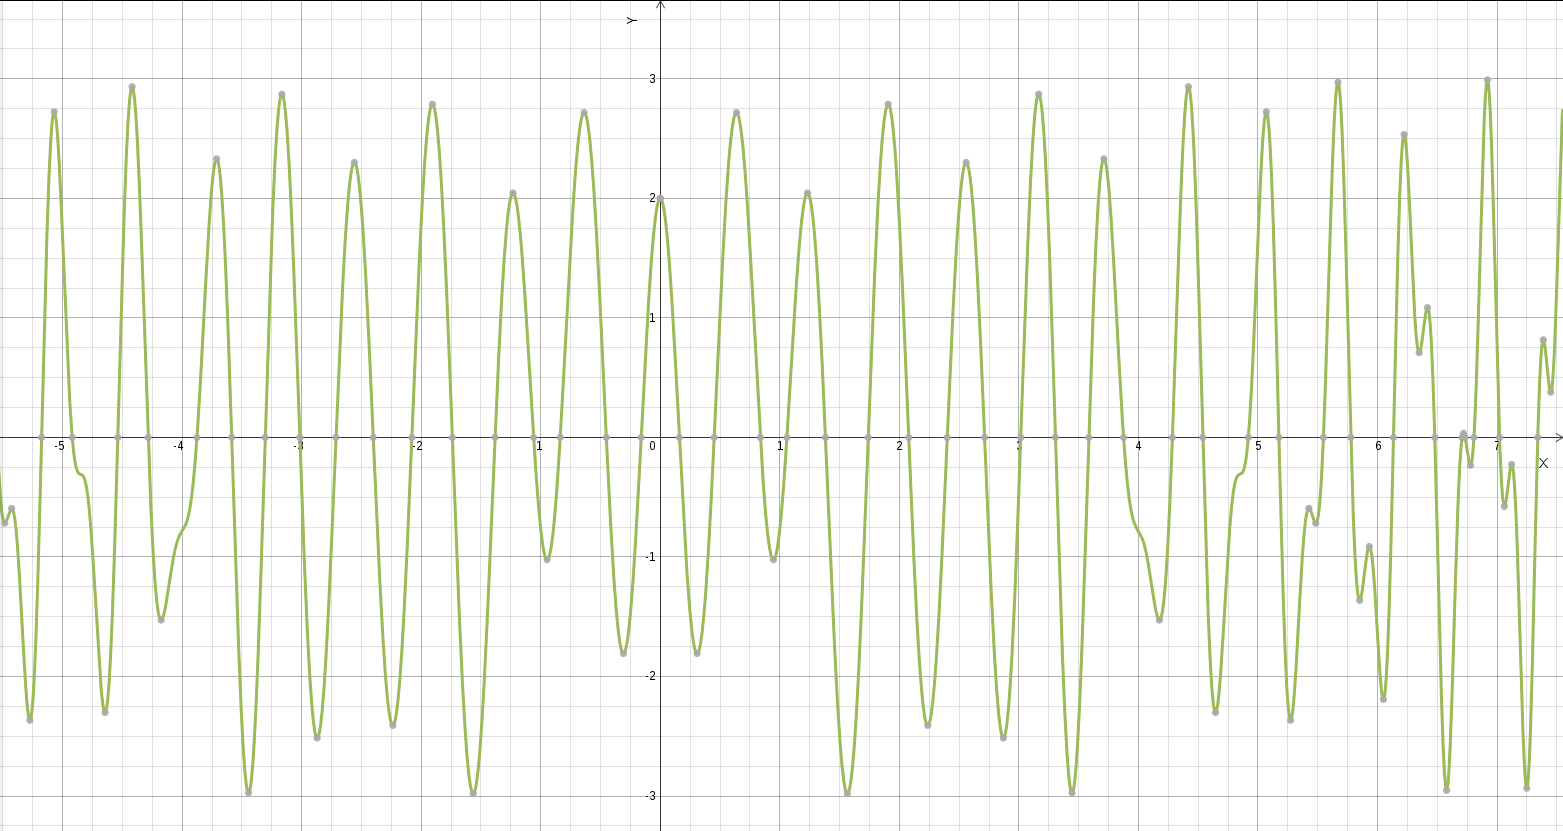
\includegraphics[width=0.9\textwidth]{science/test_function}
\caption{График тестовой функции в уравнении \ref{equation:testFunction}}
\label{figure:testFunction}
\end{figure}

Проведем измерения поколения сходимости для следующих значений количества индивидов в популяции: 2, 4, 8, 16, 32, 64, 128. Для теста возьмем значение функции сходимости равным 1000, что означает, что средняя ошибка решения должна составлять 0.03, а границы измерений возьмем от $-20$ до $20$ с количеством точек измерений равным 100. Ниже (рис.~\ref{figure:histogram2}, рис.~\ref{figure:histogram4}, рис.~\ref{figure:histogram8}, рис.~\ref{figure:histogram16}, рис.~\ref{figure:histogram32}, рис.~\ref{figure:histogram64}, рис.~\ref{figure:histogram128}) представлены гистограммы полученных результатов.

\begin{figure}[h!]
\centering
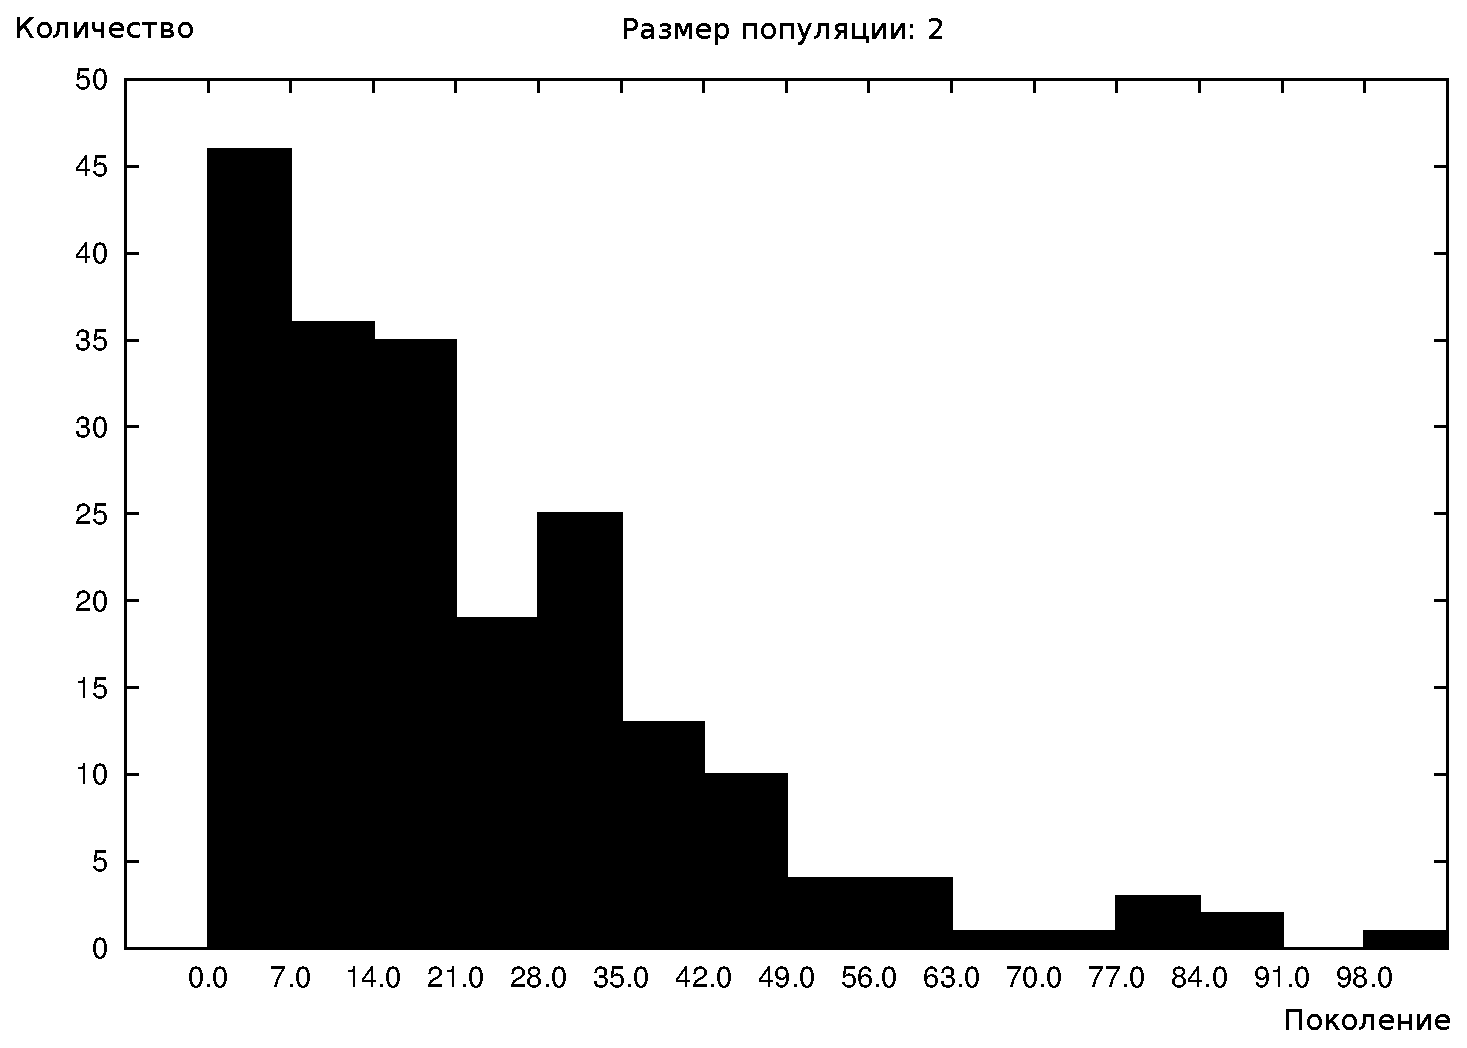
\includegraphics[width=0.8\textwidth]{science/histogram2}
\caption{Гистограмма поколения сходимости при размере популяции 2}
\label{figure:histogram2}
\end{figure}

\begin{figure}[h!]
\centering
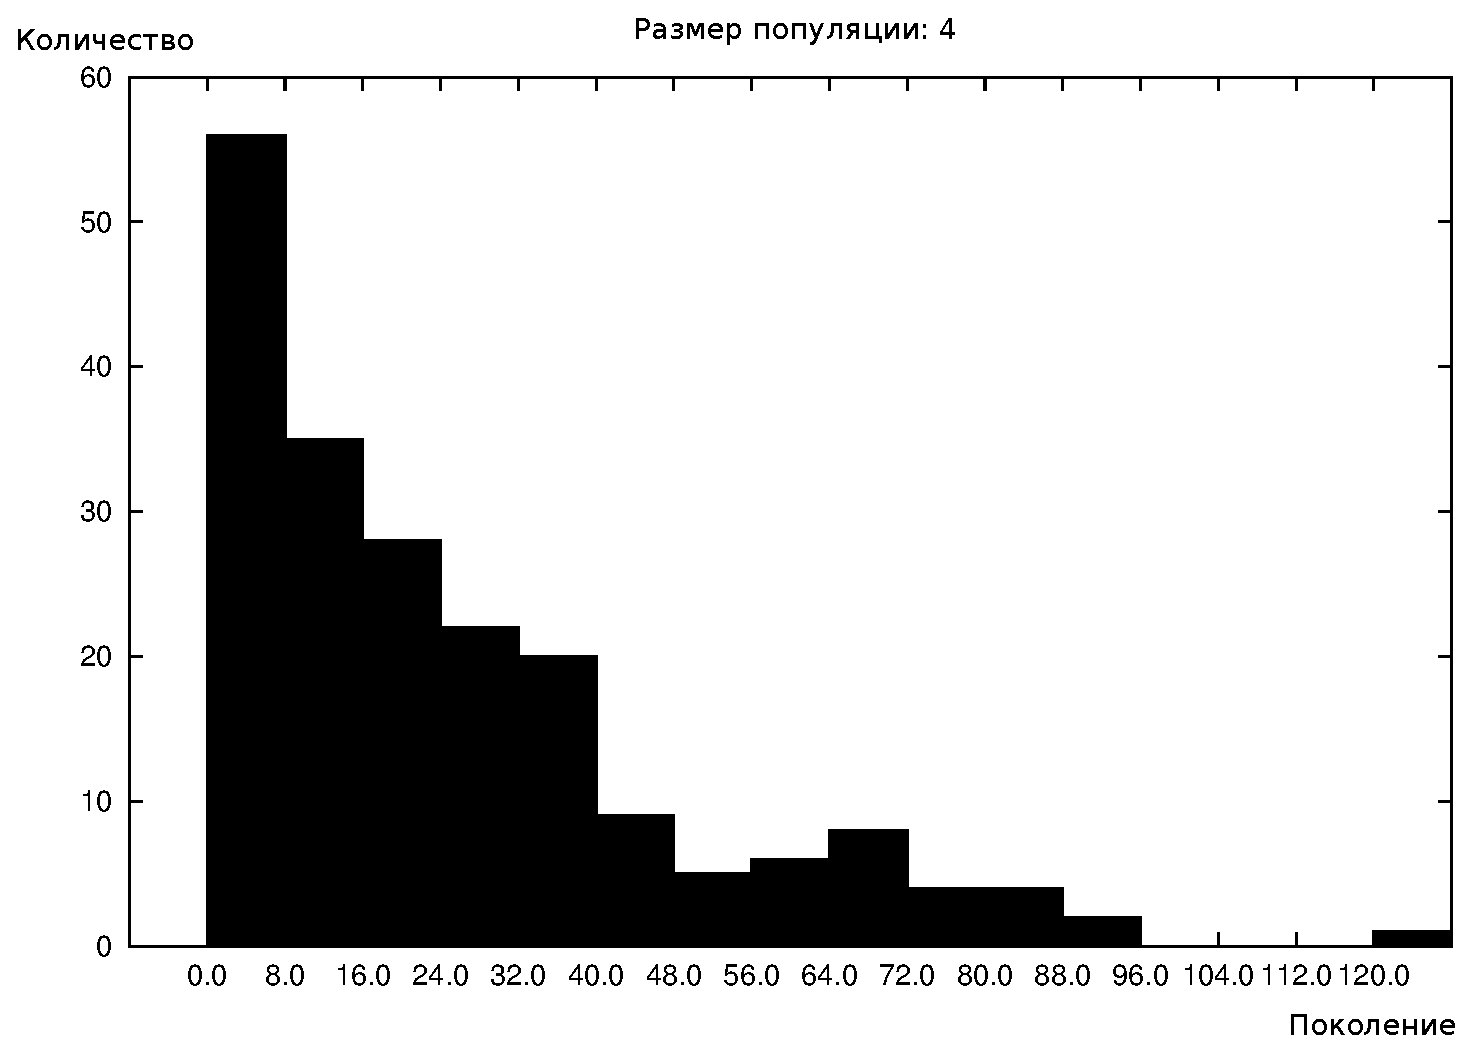
\includegraphics[width=0.8\textwidth]{science/histogram4}
\caption{Гистограмма поколения сходимости при размере популяции 4}
\label{figure:histogram4}
\end{figure}

\begin{figure}[h!]
\centering
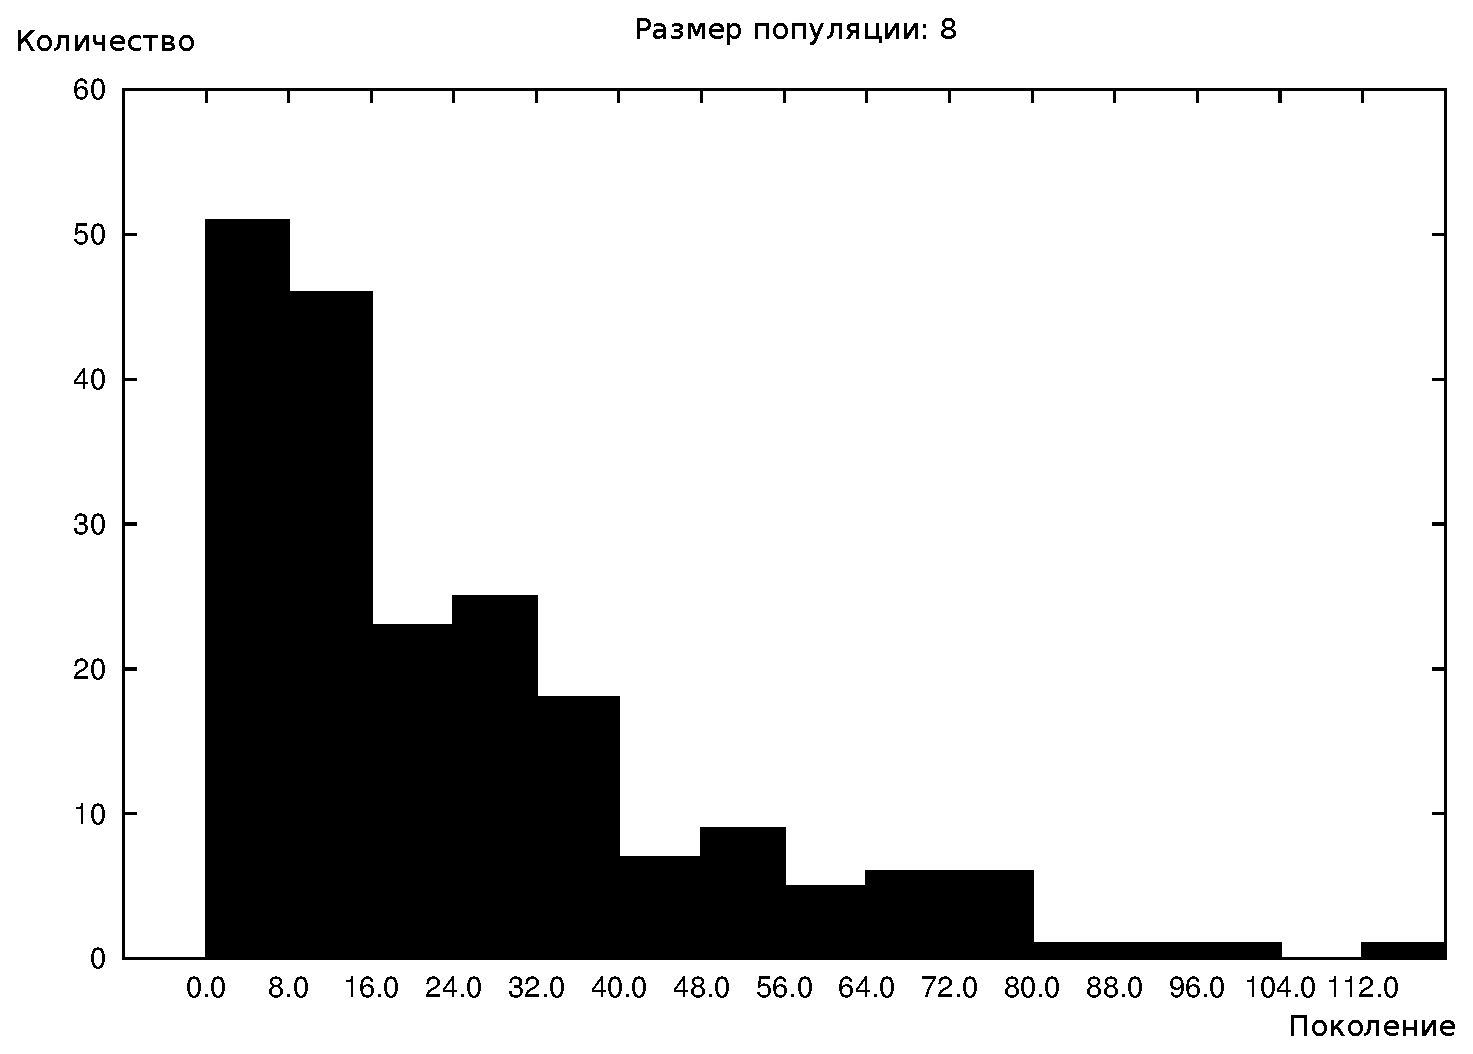
\includegraphics[width=0.8\textwidth]{science/histogram8}
\caption{Гистограмма поколения сходимости при размере популяции 8}
\label{figure:histogram8}
\end{figure}

\begin{figure}[h!]
\centering
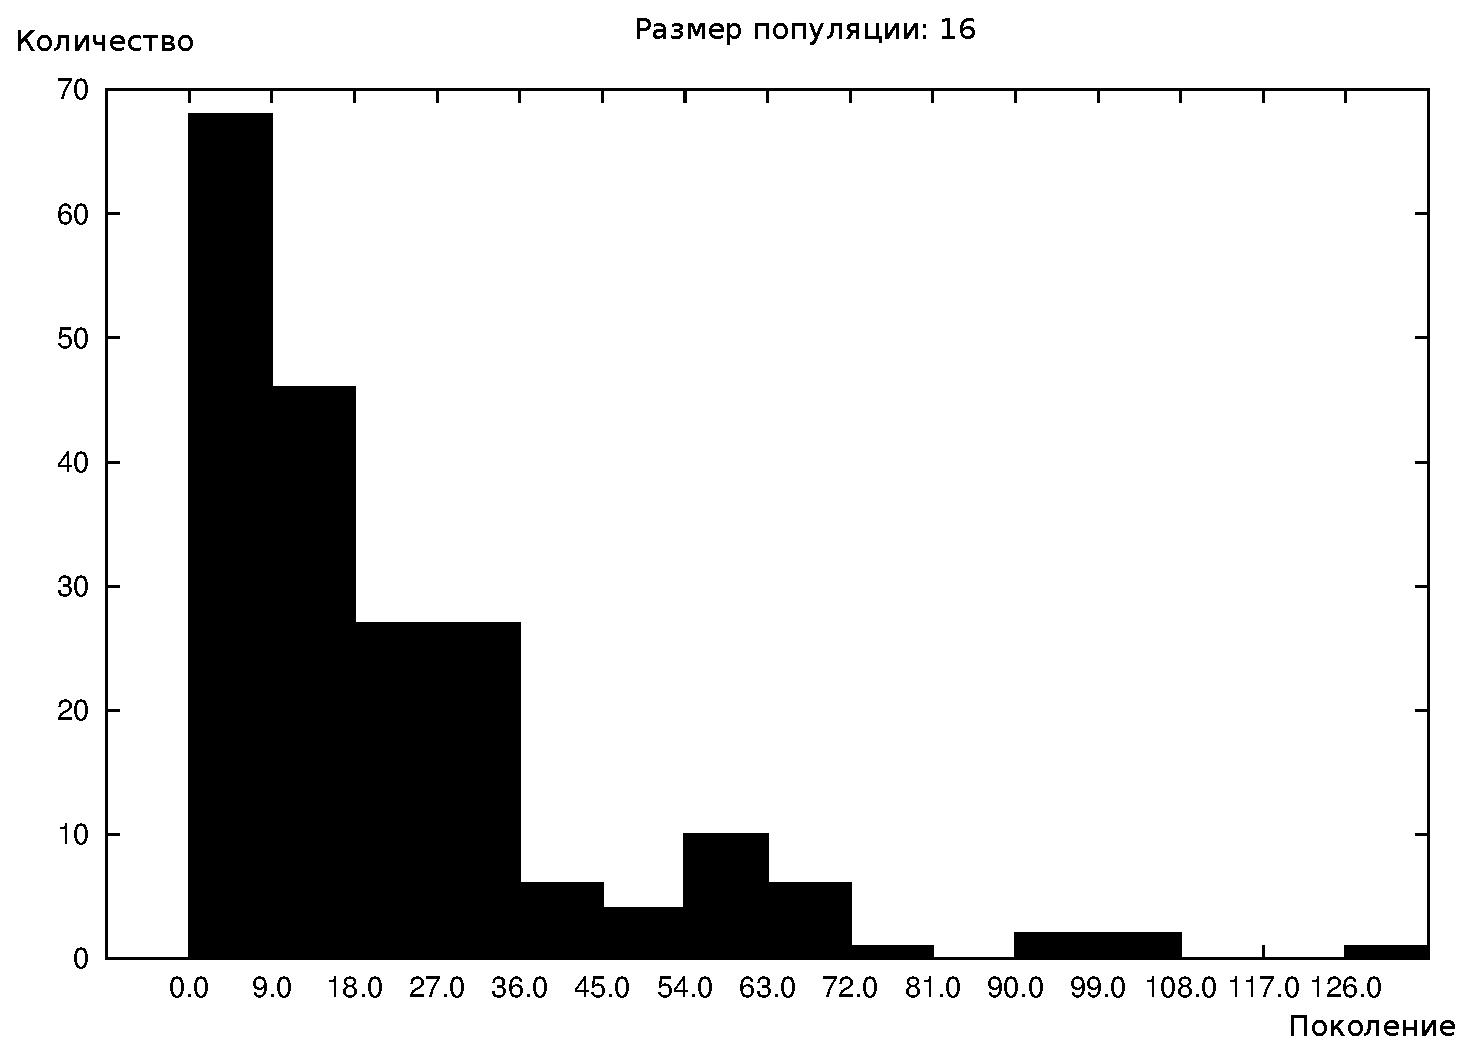
\includegraphics[width=0.8\textwidth]{science/histogram16}
\caption{Гистограмма поколения сходимости при размере популяции 16}
\label{figure:histogram16}
\end{figure}

\begin{figure}[h!]
\centering
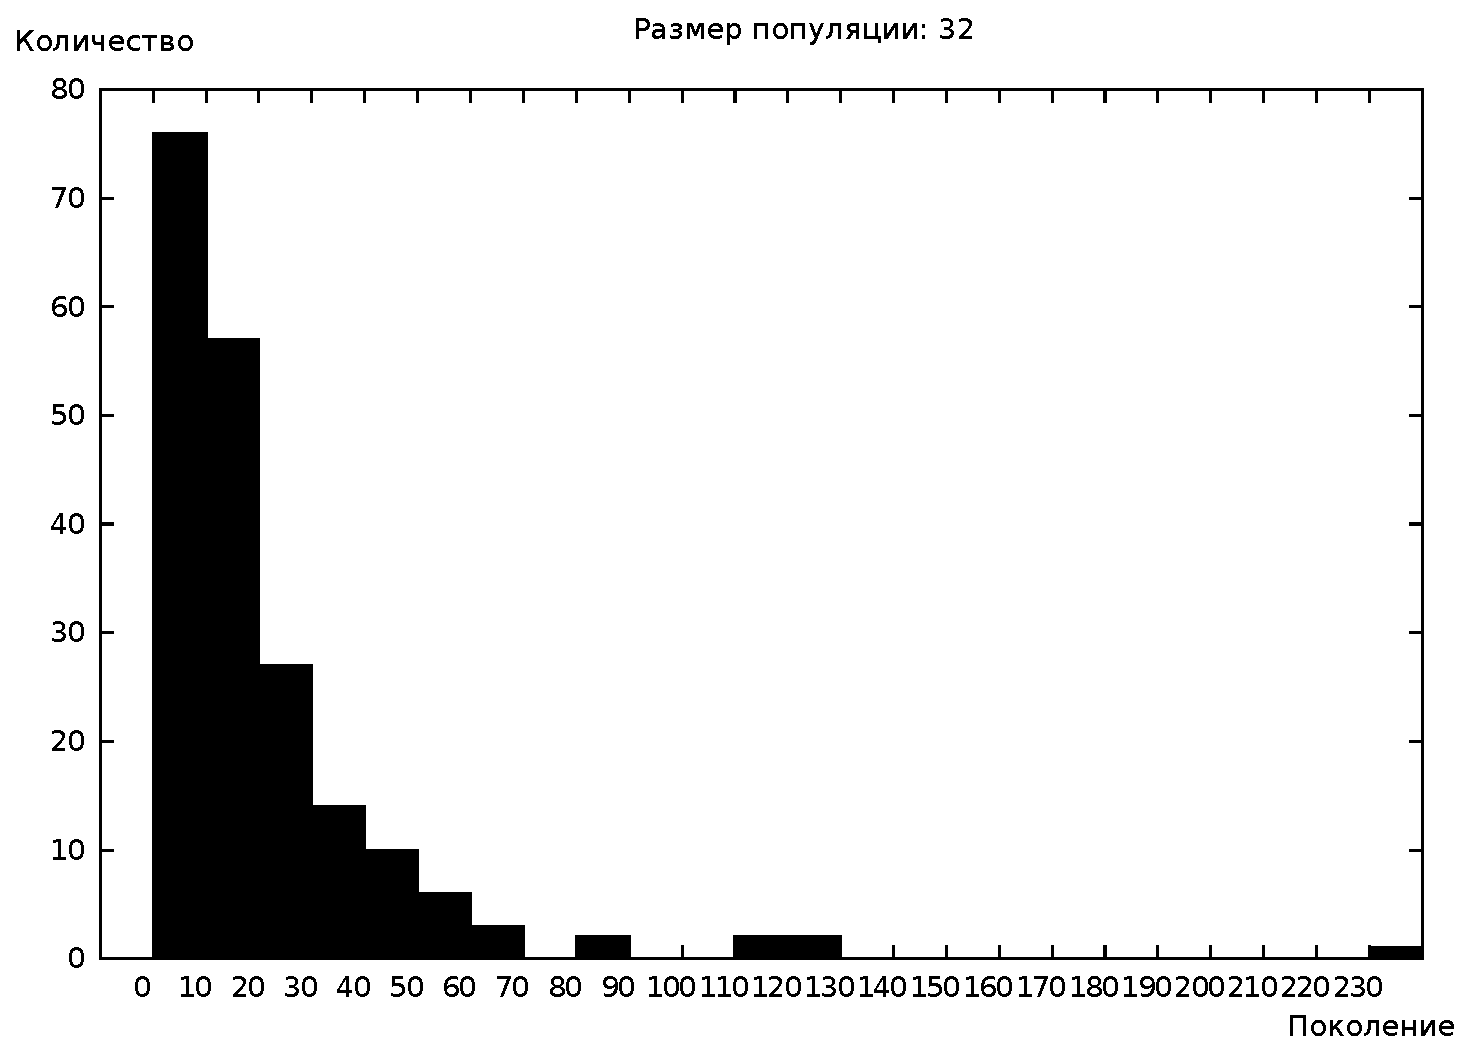
\includegraphics[width=0.8\textwidth]{science/histogram32}
\caption{Гистограмма поколения сходимости при размере популяции 32}
\label{figure:histogram32}
\end{figure}

\begin{figure}[h!]
\centering
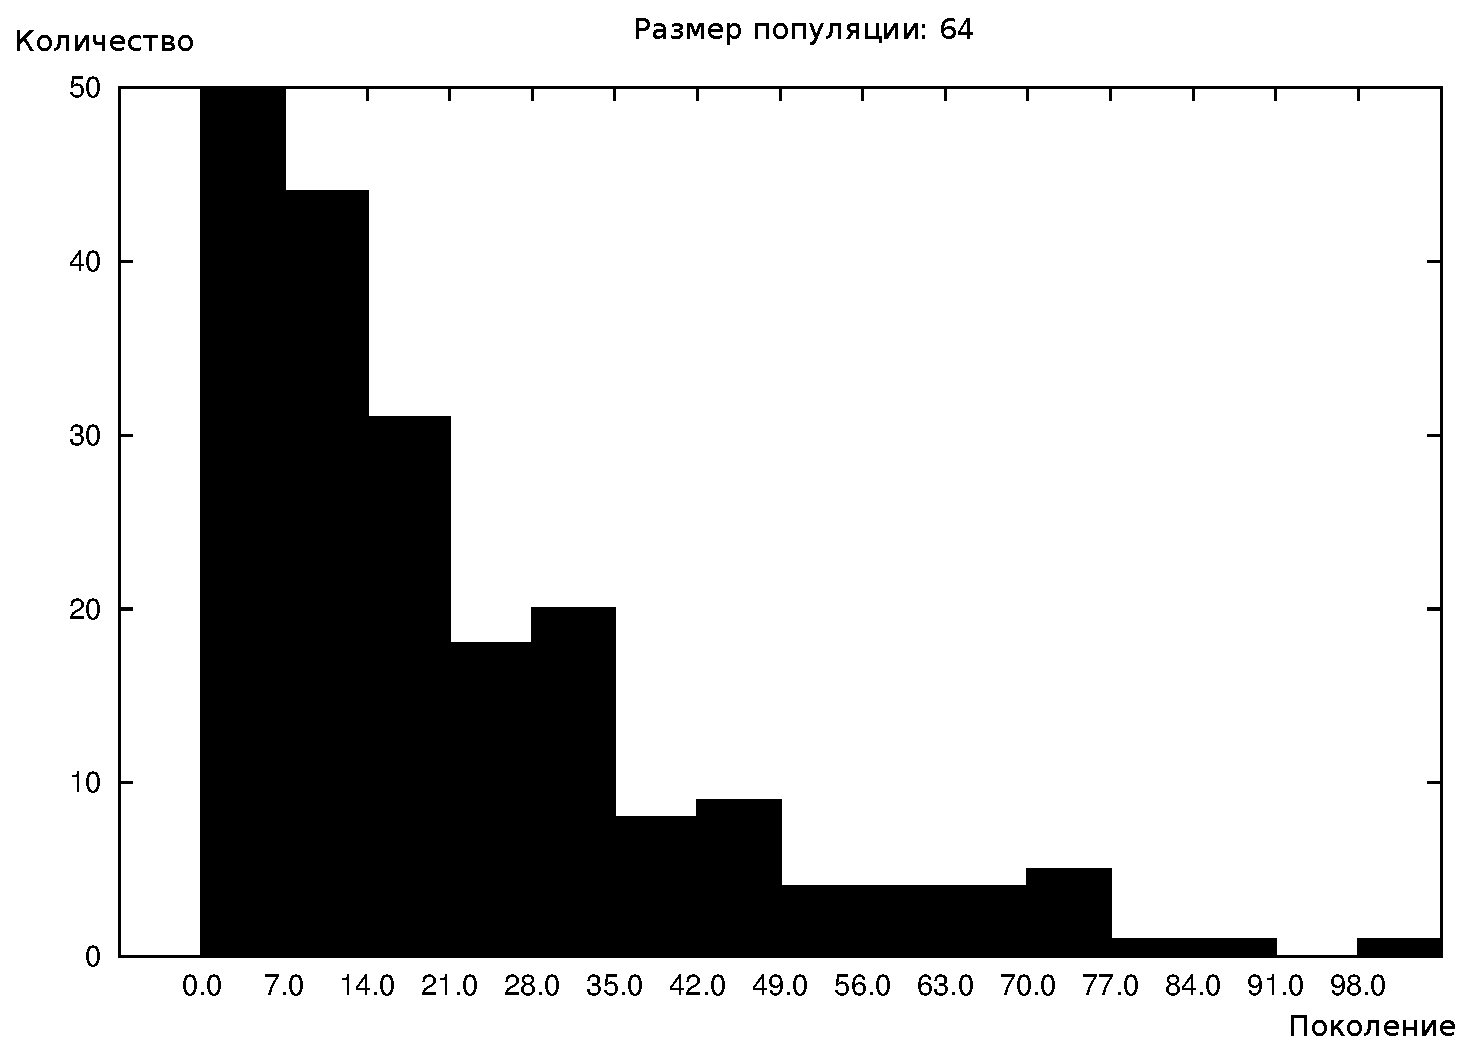
\includegraphics[width=0.8\textwidth]{science/histogram64}
\caption{Гистограмма поколения сходимости при размере популяции 64}
\label{figure:histogram64}
\end{figure}

\begin{figure}[h!]
\centering
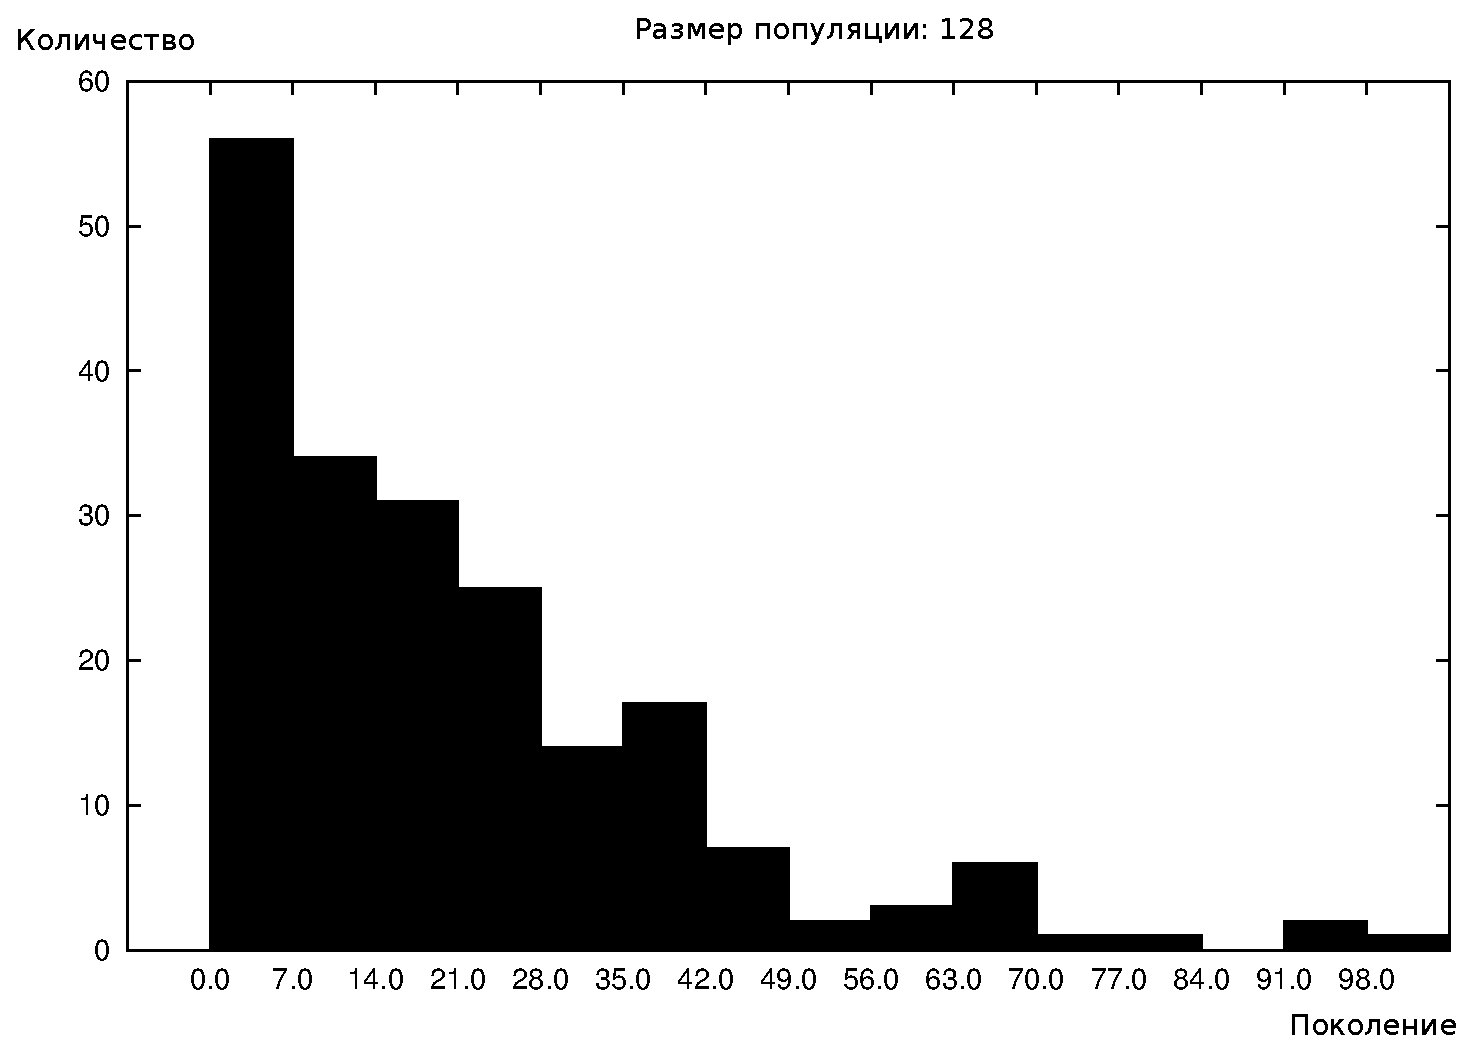
\includegraphics[width=0.8\textwidth]{science/histogram128}
\caption{Гистограмма поколения сходимости при размере популяции 128}
\label{figure:histogram128}
\end{figure}

\clearpage
\subsubsection{Определение распределения}

Анализируя гистограммы (рис.~\ref{figure:histogram2}, рис.~\ref{figure:histogram4}, рис.~\ref{figure:histogram8}, рис.~\ref{figure:histogram16}, рис.~\ref{figure:histogram32}, рис.~\ref{figure:histogram64}, рис.~\ref{figure:histogram128}), я провел исследования на соответствие известным функциям распределения с помощью теста Колмогорова-Смирнова~\cite{KolmogorovSmirnov}~\cite{BlueStatistics}.

Нулевая гипотеза:
\begin{equation}
\label{equation:distrHyp0}
H_0: \; F(t) = F_0(\frac{t}{a};\theta), \; \theta \in \Theta, \; a \in A
\end{equation}

Альтернативная гипотеза:
\begin{equation}
\label{equation:distrHyp1}
H_1: \; F(t) \neq F_0(\frac{t}{a};\theta), \; \text{для некоторых} \; \theta \in \Theta, \; a \in A
\end{equation}

В качестве функции распределения были рассмотрены следующие законы распределения:
\begin{enumerate}
\item Хи-квадрат $\chi^2(1)$;
\item Хи-квадрат $\chi^2(2)$;
\item Распределение Фишера $F(1, 1)$;
\item Гамма распределение $\Gamma(1, 2.0)$;
\item Распределение Коши $F_X(0.5)$;
\end{enumerate}

Проверка распределений проводилась на значениях размера популяций в 16, 32 и 64 индивида. Размер выборки брался 1000 элементов. Так как поставленная гипотеза является сложной и тест Колмогорова перестает быть независимым от распределения, разобьем задачу на две. 

Исходя из гистограмм распределения зададим границы множества $a \in A$:
\begin{equation}
a_{min} \leq a \leq a_{max}
\end{equation}

Разобьем полученный интервал на $N = 1000$ частей и для каждой точки:
\begin{equation}
a(i) = a_{min} + i \cdot \frac{a_{max} - a_{min}}{N}, i \in \overline{0 .. N}
\end{equation}

Проведем проверку простой гипотезы:
\begin{equation}
\label{equation:distrHyp0Simple}
H_0': \; F(t) = F_0(\frac{t}{a(i)};\theta), \; \theta \in \Theta
\end{equation}

Против альтернативной гипотезы:
Проведем проверку простой гипотезы:
\begin{equation}
\label{equation:distrHyp1Simple}
H_1': \; F(t) \neq F_0(\frac{t}{a(i)};\theta), \; \text{для некоторых} \; \theta \in \Theta
\end{equation}

Выберем значение ошибки первого рода:
\begin{equation}
\alpha = 0.05
\end{equation}

Статистика $D(\vec{X}_n)$ критерия Колмогорова реализуется как:
\begin{equation}
D(\vec{x}_n) = sup_t | F_n(t) - F_0(t) |
\end{equation}
\begin{ESKDExplanation}
\item[где ] $F_n(t)$ -- эмпирическая функция распределения, построенная по реализации $\vec{x}_n$ случайной выборки $\vec{X}_n$.
\end{ESKDExplanation}

Так как мы задали значение ошибки первого рода, то мы отклоняем гипотезу $H_0'$ при:
\begin{equation}
D(\vec{x}_n) > D_{1 - \alpha}
\end{equation}
\begin{ESKDExplanation}
\item[где ] $D_{1 - \alpha}$ -- квантиль уровня $1 - \alpha$ распределения случайно величины $D(\vec{x}_n)$ при условии истинности основной гипотезы $H_0'$.
\end{ESKDExplanation}

Согласно~\cite{BlueStatistics}:
\begin{equation}
D_{1 - \alpha} \approx \frac{t_{1 - \alpha}}{\sqrt{n}}
\end{equation}

Где величина $t_{1 - \alpha}$ определяется:
\begin{equation}
K(t) = \sum_{k = - \inf}^{\inf} (-1)^k e^{-2 k^2 t^2}, \; K(t_{1-\alpha}) =  1 - \alpha
\end{equation}

Вычисление значения функции $K(t)$ ведется либо по таблицам, либо с помощью метода, приведенного в работе~\cite{KolmogorovSmirnov}.

Значения $D(\vec{x}_n)$ вычисляются~\cite{BlueStatistics} по следующей приближенной формуле:
\begin{equation}
D(\vec{x}_n) = \max_{1 \leq i \leq n} \left ( \left | F_0(x_{(i)}) - \frac{2i - 1}{2n} \right | + \frac{1}{2n}  \right )
\end{equation}
\begin{ESKDExplanation}
\item[где ] $x_{(i)}, i = \overline{1,n}$ -- члены вариационного ряда, построенного по выборке $x_1, ..., x_n$.
\end{ESKDExplanation}

\subsubsection{Результаты исследования}
В результате работы данного алгоритма я получил следующие результаты:
\begin{itemize}
\item Распределение поколения сходимости для фиксированного значения функции приспособленности соответствует смещенное распределение хи-квадрат $\chi^2(2)$ с параметром равным 2. При малых размерах выборки также подходит смещенное распределение хи-квадрат $\chi^2(1)$, но данное распределение расходится с экспериментальными данными уже при размерах выборки $n = 70$.
\item Значения параметра $a$ для смещения распределения при заданном уровне достоверности $\alpha = 0.05$ колеблется в интервале $8 < a < 12$ в зависимости от размеров популяции.
\item Значение параметра $a$ зависит от размеров популяции (количеств индивидов в ней), а также от вида функции, которая используется для генерации входных данных для символьной регрессии на основе разработанного эволюционного алгоритма.
\item Практическое значение результата заключается в том, что разработанный алгоритм в принципе сходится и дает хорошие результаты за приемлимое время.
\item Теоретическое значение результата заключается в появившейся теоретической модели работы символьной регрессии на основе эволюционного алгоритма, что позволяет проводить имитационное моделирование системы в составе крупных комплексов.
\end{itemize}

Для отображения результатов исследовательской работы преобразуем гистограммы сходимости символьной регрессии с помощью метода Estimation of Kernel Density~\cite{KernelDensity} для получения экспериментальной функции плотности распределения и отобразим полученную теоретическую функцию плотности для смещенного распределения $\chi^2(2)$ на рис.~\ref{figure:finalDistr}. Исходная гистограмма, преобразованная для отображения экспериментальной плотности вероятности распределения, представлена на рис.~\ref{figure:finalDistrHistr}.

\begin{figure}[h!]
\centering
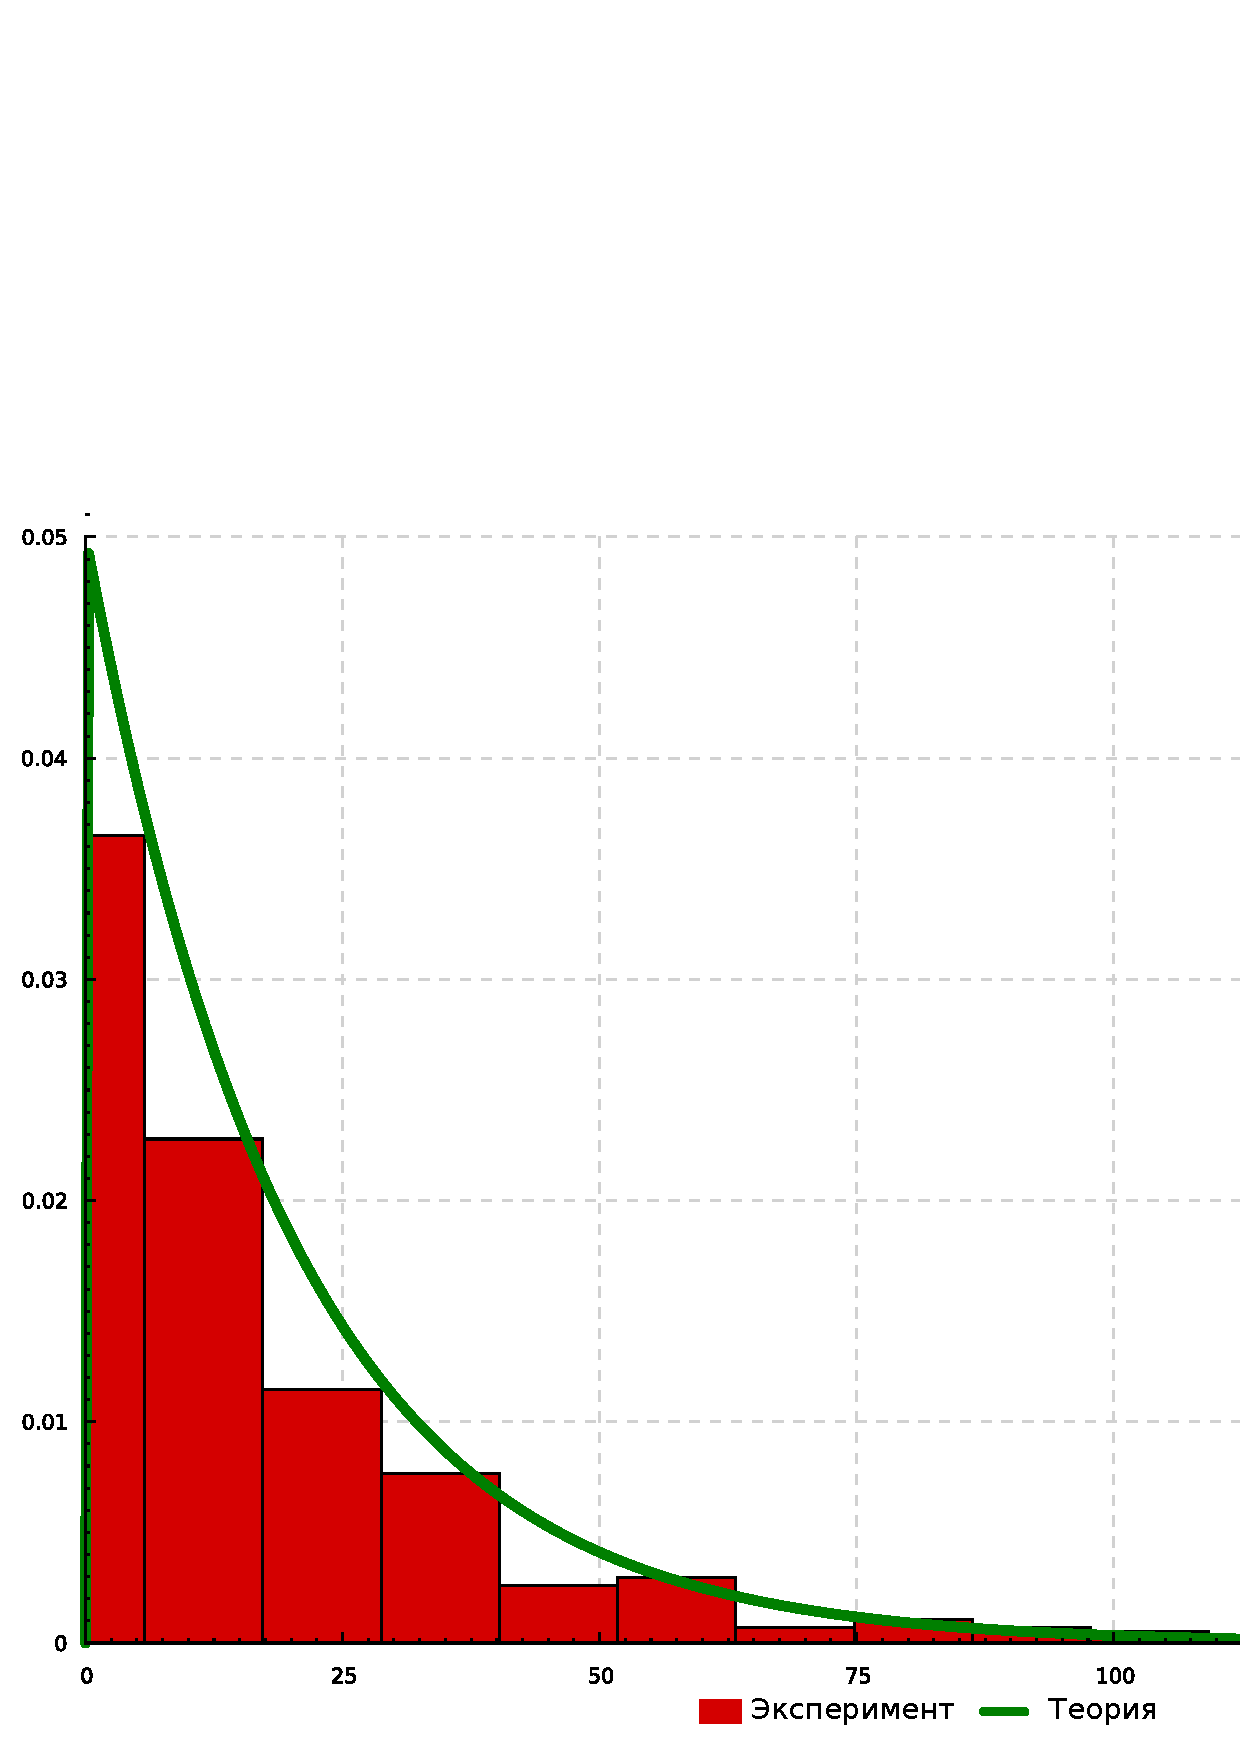
\includegraphics[width=0.91\textwidth]{science/final_hist}
\caption{Сравнение теоретической $\chi^2(2)$ функции плотности вероятности и экспериментальных данных в виде гистограммы плотности вероятности}
\label{figure:finalDistrHistr}
\end{figure}

\begin{figure}[h!]
\centering
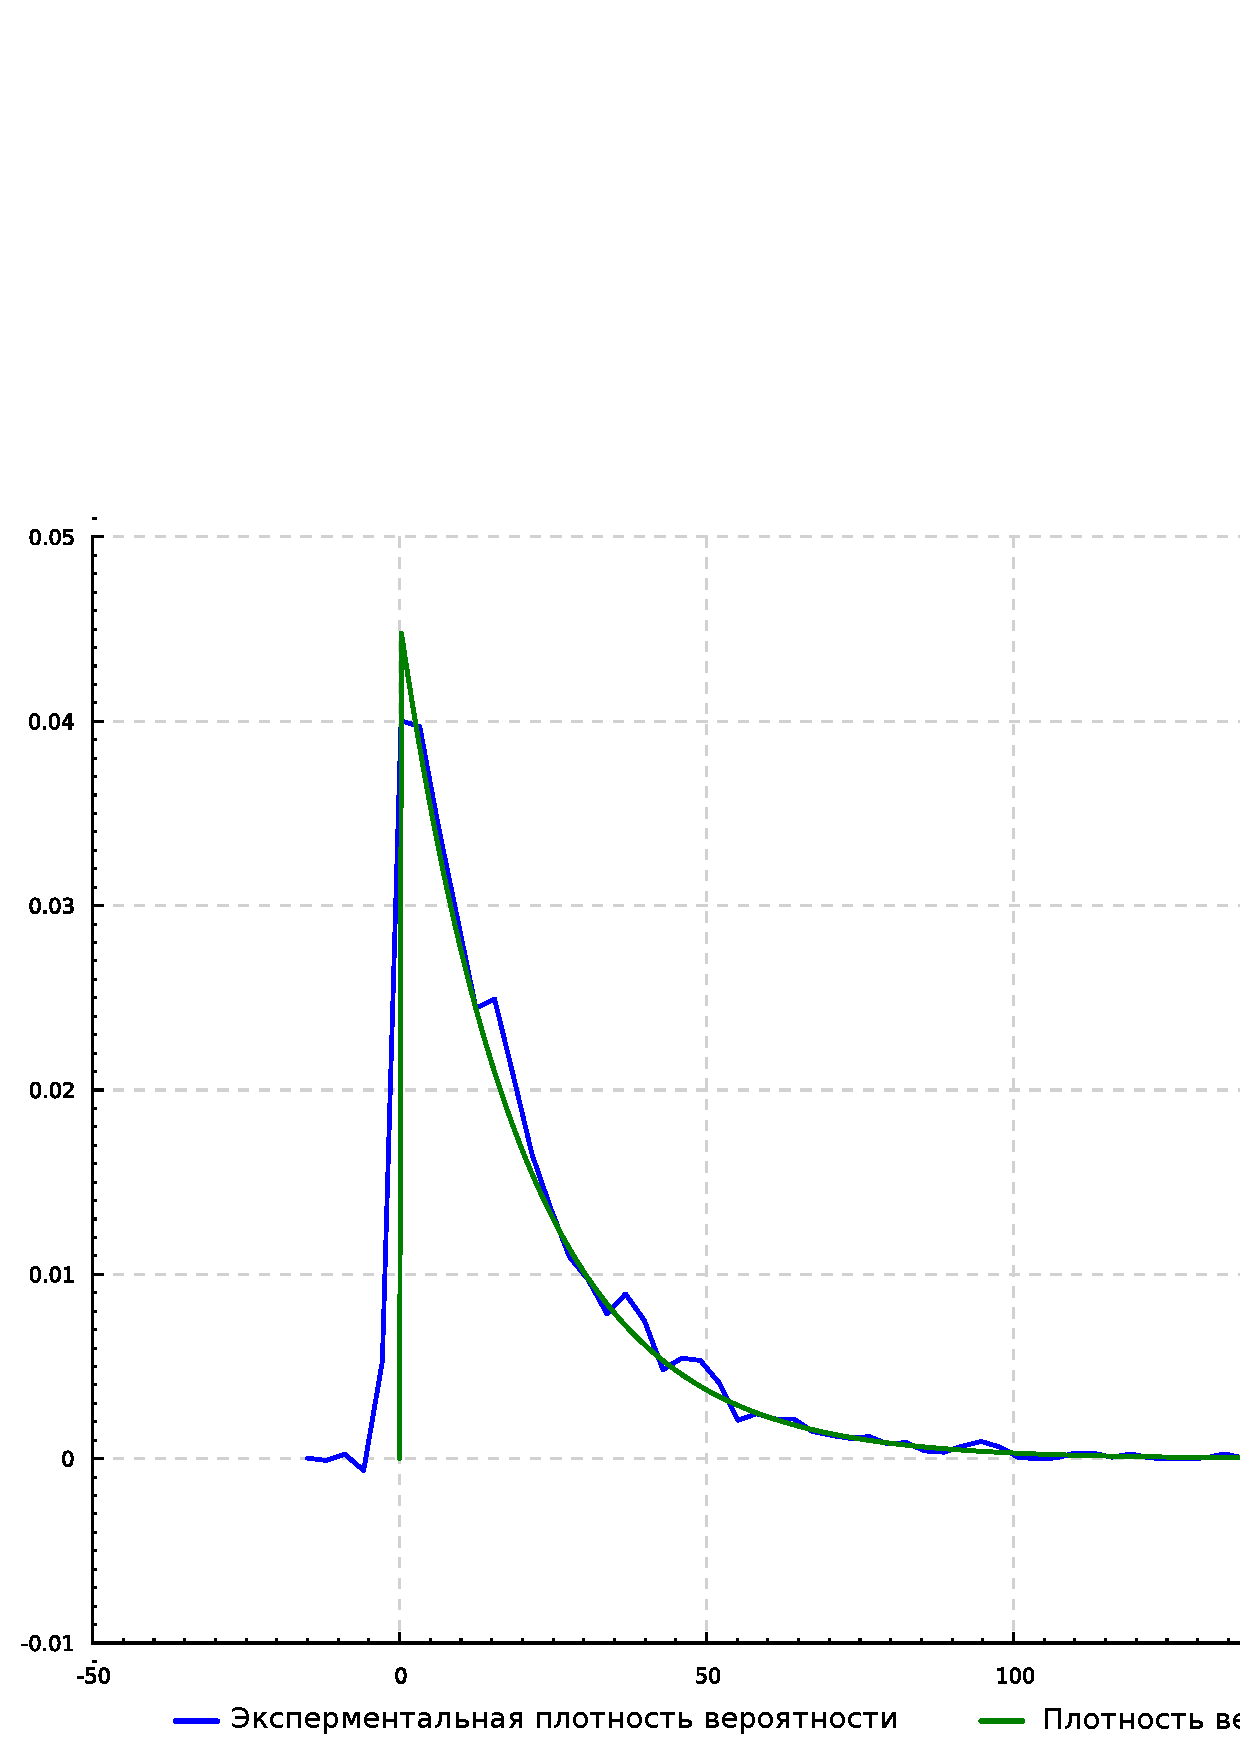
\includegraphics[width=0.91\textwidth]{science/final}
\caption{Сравнение теоретической $\chi^2(2)$ и экспериментальной функций плотности вероятности}
\label{figure:finalDistr}
\end{figure}